% $Id: template.tex 11 2007-04-03 22:25:53Z jpeltier $

%\documentclass{vgtc}                          % final (conference style)
%\documentclass[review]{vgtc}                 % review
%\documentclass[widereview]{vgtc}             % wide-spaced review
%\documentclass[preprint]{vgtc}               % preprint
\documentclass[electronic]{vgtc}             % electronic version

%% Uncomment one of the lines above depending on where your paper is
%% in the conference process. ``review'' and ``widereview'' are for review
%% submission, ``preprint'' is for pre-publication, and the final version
%% doesn't use a specific qualifier. Further, ``electronic'' includes
%% hyperreferences for more convenient online viewing.

%% Please use one of the ``review'' options in combination with the
%% assigned online id (see below) ONLY if your paper uses a double blind
%% review process. Some conferences, like IEEE Vis and InfoVis, have NOT
%% in the past.

%% Figures should be in CMYK or Grey scale format, otherwise, colour 
%% shifting may occur during the printing process.

%% These few lines make a distinction between latex and pdflatex calls and they
%% bring in essential packages for graphics and font handling.
%% Note that due to the \DeclareGraphicsExtensions{} call it is no longer necessary
%% to provide the the path and extension of a graphics file:
%% \includegraphics{diamondrule} is completely sufficient.
%%
\ifpdf%                                % if we use pdflatex
  \pdfoutput=1\relax                   % create PDFs from pdfLaTeX
  \pdfcompresslevel=9                  % PDF Compression
  \pdfoptionpdfminorversion=7          % create PDF 1.7
  \ExecuteOptions{pdftex}
  \usepackage{graphicx}                % allow us to embed graphics files
  \DeclareGraphicsExtensions{.pdf,.png,.jpg,.jpeg} % for pdflatex we expect .pdf, .png, or .jpg files
\else%                                 % else we use pure latex
  \ExecuteOptions{dvips}
  \usepackage{graphicx}                % allow us to embed graphics files
  \DeclareGraphicsExtensions{.eps}     % for pure latex we expect eps files
\fi%

%% it is recomended to use ``\autoref{sec:bla}'' instead of ``Fig.~\ref{sec:bla}''
\graphicspath{{figures/}{pictures/}{images/}{./}} % where to search for the images

\usepackage{microtype}                 % use micro-typography (slightly more compact, better to read)
\PassOptionsToPackage{warn}{textcomp}  % to address font issues with \textrightarrow
\usepackage{textcomp}                  % use better special symbols
\usepackage{mathptmx}                  % use matching math font
\usepackage{times}                     % we use Times as the main font
\renewcommand*\ttdefault{txtt}         % a nicer typewriter font
\usepackage{cite}                      % needed to automatically sort the references
\usepackage{tabu}                      % only used for the table example
\usepackage{booktabs}                  % only used for the table example
%% We encourage the use of mathptmx for consistent usage of times font
%% throughout the proceedings. However, if you encounter conflicts
%% with other math-related packages, you may want to disable it.


%% If you are submitting a paper to a conference for review with a double
%% blind reviewing process, please replace the value ``0'' below with your
%% OnlineID. Otherwise, you may safely leave it at ``0''.
\onlineid{0}

%% declare the category of your paper, only shown in review mode
\vgtccategory{Summary}

%% allow for this line if you want the electronic option to work properly
\vgtcinsertpkg

%% In preprint mode you may define your own headline.
%\preprinttext{To appear in an IEEE VGTC sponsored conference.}

%% Paper title.

\title{Survey: Visual Analysis Approaches to Time Series Prediction}

%% This is how authors are specified in the conference style

%% Author and Affiliation (single author).
\author{Fabian Otto\thanks{e-mail: fabian.otto@stud.tu-darmstadt.de}}
\affiliation{\scriptsize Technical University Darmstadt}

%% A teaser figure can be included as follows, but is not recommended since
%% the space is now taken up by a full width abstract.
%\teaser{
%  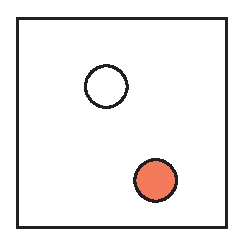
\includegraphics[width=1.5in]{sample.eps}
%  \caption{Lookit! Lookit!}
%}

%% Abstract section.
\abstract{
	
} % end of abstract

% \nocopyrightspace

%%%%%%%%%%%%%%%%%%%%%%%%%%%%%%%%%%%%%%%%%%%%%%%%%%%%%%%%%%%%%%%%
%%%%%%%%%%%%%%%%%%%%%% START OF THE PAPER %%%%%%%%%%%%%%%%%%%%%%
%%%%%%%%%%%%%%%%%%%%%%%%%%%%%%%%%%%%%%%%%%%%%%%%%%%%%%%%%%%%%%%%%

\begin{document}

\firstsection{Introduction}

\maketitle

% rewrite
Predictive analytics is concerned with the prediction of future probabilities and trends based on observed events. 
It encompasses a multi-perspective approach that includes integrated reasoning, pattern recognition and predictive modeling associated with domain knowledge.
However, the primary use of such systems tends to be reactive, meaning that analytic systems are typically
% spatial
In spatiotemporal data, analysts are searching for regions of space and time with unusually high incidences of events.
In the cases that hotspots are found, analysts would like to predict how these regions may grow in order to plan decision support and preventative measures.
Furthermore, analysts would also like to predict where future hotspots may occur.

\section{Temporal Time Series \label{sec:temporal}}
content 

\subsection{Simple Time Series \label{subsec:simple}}
content

\subsection{Time Series Prediction with Peak Preservation \label{subsec:peak}}
content

\subsection{Multivariate Time Series \label{subsec:multivar}}
Visual Analytics approaches for simple time series prediction (\autoref{subsec:simple}) offer a great variety for single time series.
However, in a practical environment it is often necessary to evaluate multiple time series in parallel or deal with multidimensional input variables.
In order to solve these problems, visual analytics approaches for simple time series are not sufficient anymore.\\ 
An older Visual Analytics approaches for multivariate time series prediction is from Ichikawa et al. \cite{ichikawa:2002}.
Their goal was to predict multiple daytime stock prices and simultaneously visualize a set of prediction from different simulation systems within a single system. 
Therefore, their system supports multiple prediction for a single stock as well as predictions of multiple stocks. 
One major finding was, visualizing multivariate predictions in a 3-dimensional space creates large amounts of occlusion, thus it is not suitable.
Instead the system utilizes line charts with cluttering control and color charts with level-of-detail control. 
The line charts support multivariate scaling, i.e. the time axis of the plot can be scaled differently to focus one certain areas, e.g. with less overlap.
Further, the lines are colored differently, depending on the amount of overlap/uniform predictions.
The color chart is composed of horizontal color-bands for each prediction, whereas a vertical color band can be seen as a period in time. 
In order to improve the visualization, the different color-bands are cluster based on the user-specified level-of detail. 
This results in a smaller amount of horizontal color-bands where the individual properties are diminished. 
In the workspace the above plots can be displayed with different axis.
This enables the user to compare a set of predictions for different parameter ranges (e.g. sales organizations) as well as different stocks simultaneously.
Consequently, the user can get a overview or trend, but due to clustering and simply the amount of predictions displayed, he can hardly extract specific information.\\


\subsection{Pattern and Anomaly Detection\label{subsec:pattern}}

Another system can be found from Steed et al. \cite{steed:2017}.
Their approach is focused on understanding patterns in log and imagery data collected by 3D printers.

%\begin{figure}[tb]
% \centering
% 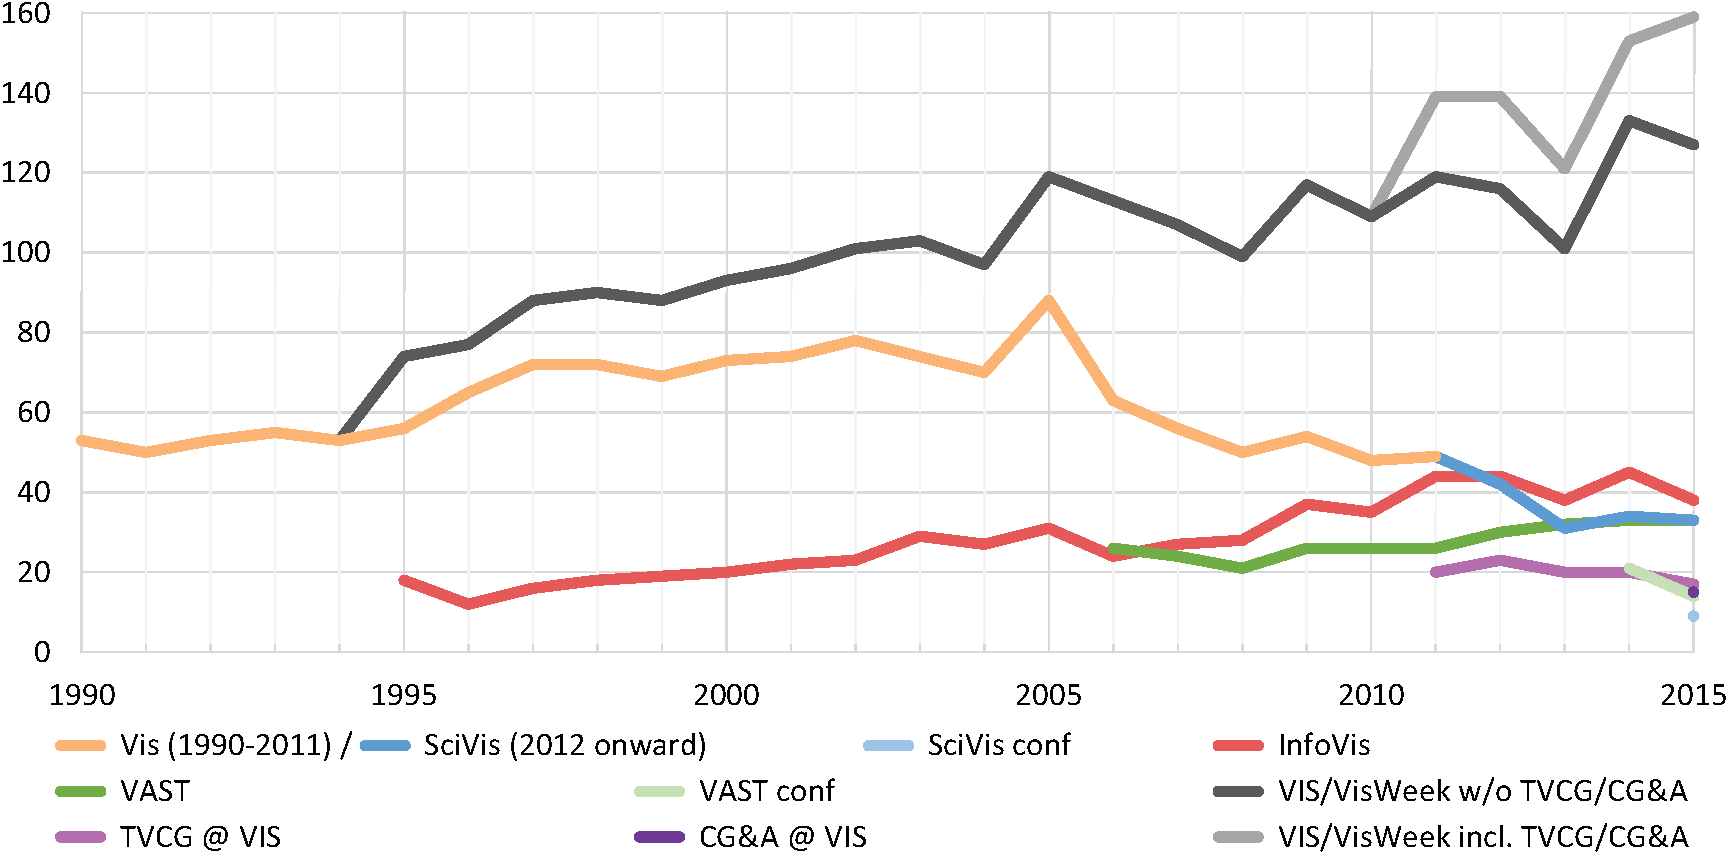
\includegraphics[width=\columnwidth]{paper-count-w-2015-new}
% \caption{A visualization of the 1990--2015 data from . The image is from and is in the public domain.}
% \label{fig:sample}
%\end{figure}

\section{Spatiotemporal Time Series\label{sec:spatiotemp}}

% TODO
\cite{yue:2009}

The previous section (\autoref{sec:temporal}) presented an overview of systems for temporal time series prediction as well as pattern and anomaly detection. 
However, in other application areas such as crime prevention as well as emergency and epidemic intelligence, not only the temporal data is of value, but also locations. 
Typically, these locations fit into a hierarchical categorization structure, which can be filtered.
Further, the data categories are processed either as aggregated time series over a spatial location (e.g. county, zip code, collection station) or represent a spatial snapshots of a small time aggregate (e.g., day, week).\\
One system which focuses on spatiotemporal prediction is from Maciejewski et al. \cite{maciejewski:2011}.
It is based on their previous work \cite{maciejewski:2008, maciejewski:2007} and centers around on categorical geospatiotemporal event data, where events consist of locations
in time and/or space, and each event fits into a hierarchical categorization structure.
Specifically, they used a data set for detecting adverse health events using pre-diagnosis information from emergency departments.
The system itself provides a colored geospatial window, which shows the percentage of events in a certain area, e.g. patients at an emergency department, which where classified with respiratory syndromes.
Further, the user is able to apply filtering on a fine and coarse-grained level. 
The systems also differentiates between the time series and the geospatial prediction.
The time series prediction is achieved by cumulative summation or a seasonal-trend decomposition based on locally weighted regression.
%spatially aggregating the data, e.g. for one state, etc.
For multivariate data, each event category is modeled as a separate time series signal. 
Equivalent to the time series prediction, the granularity/level of aggregation (e.g. state, county, etc.) for geospatial predictions can be adjusted by the user.
Further, the system provides a Kernel Density Estimation approach which allows to display the spatiotemporal distribution on a more fine-grained level.
In order to detect anomalies, e.g. outbreaks, (also see \autopageref{subsec:pattern}) the system calculates the difference between the predicted and the actual values and highlights areas above a user specified threshold.

\section{Conclusion}
content

%\bibliographystyle{abbrv}
%\bibliographystyle{abbrv-doi}
%\bibliographystyle{abbrv-doi-narrow}
\bibliographystyle{abbrv-doi-hyperref}
%\bibliographystyle{abbrv-doi-hyperref-narrow}

\bibliography{bibliography}
\end{document}
